\documentclass[border=10pt]{standalone}
\usepackage[svgnames]{xcolor}
\usepackage{amsmath}
\usepackage{pgfplots}
\pgfplotsset{compat=newest}
\usepackage[sfdefault]{FiraSans}
\usepackage{FiraMono}
\renewcommand*\familydefault{\sfdefault}
\begin{document}
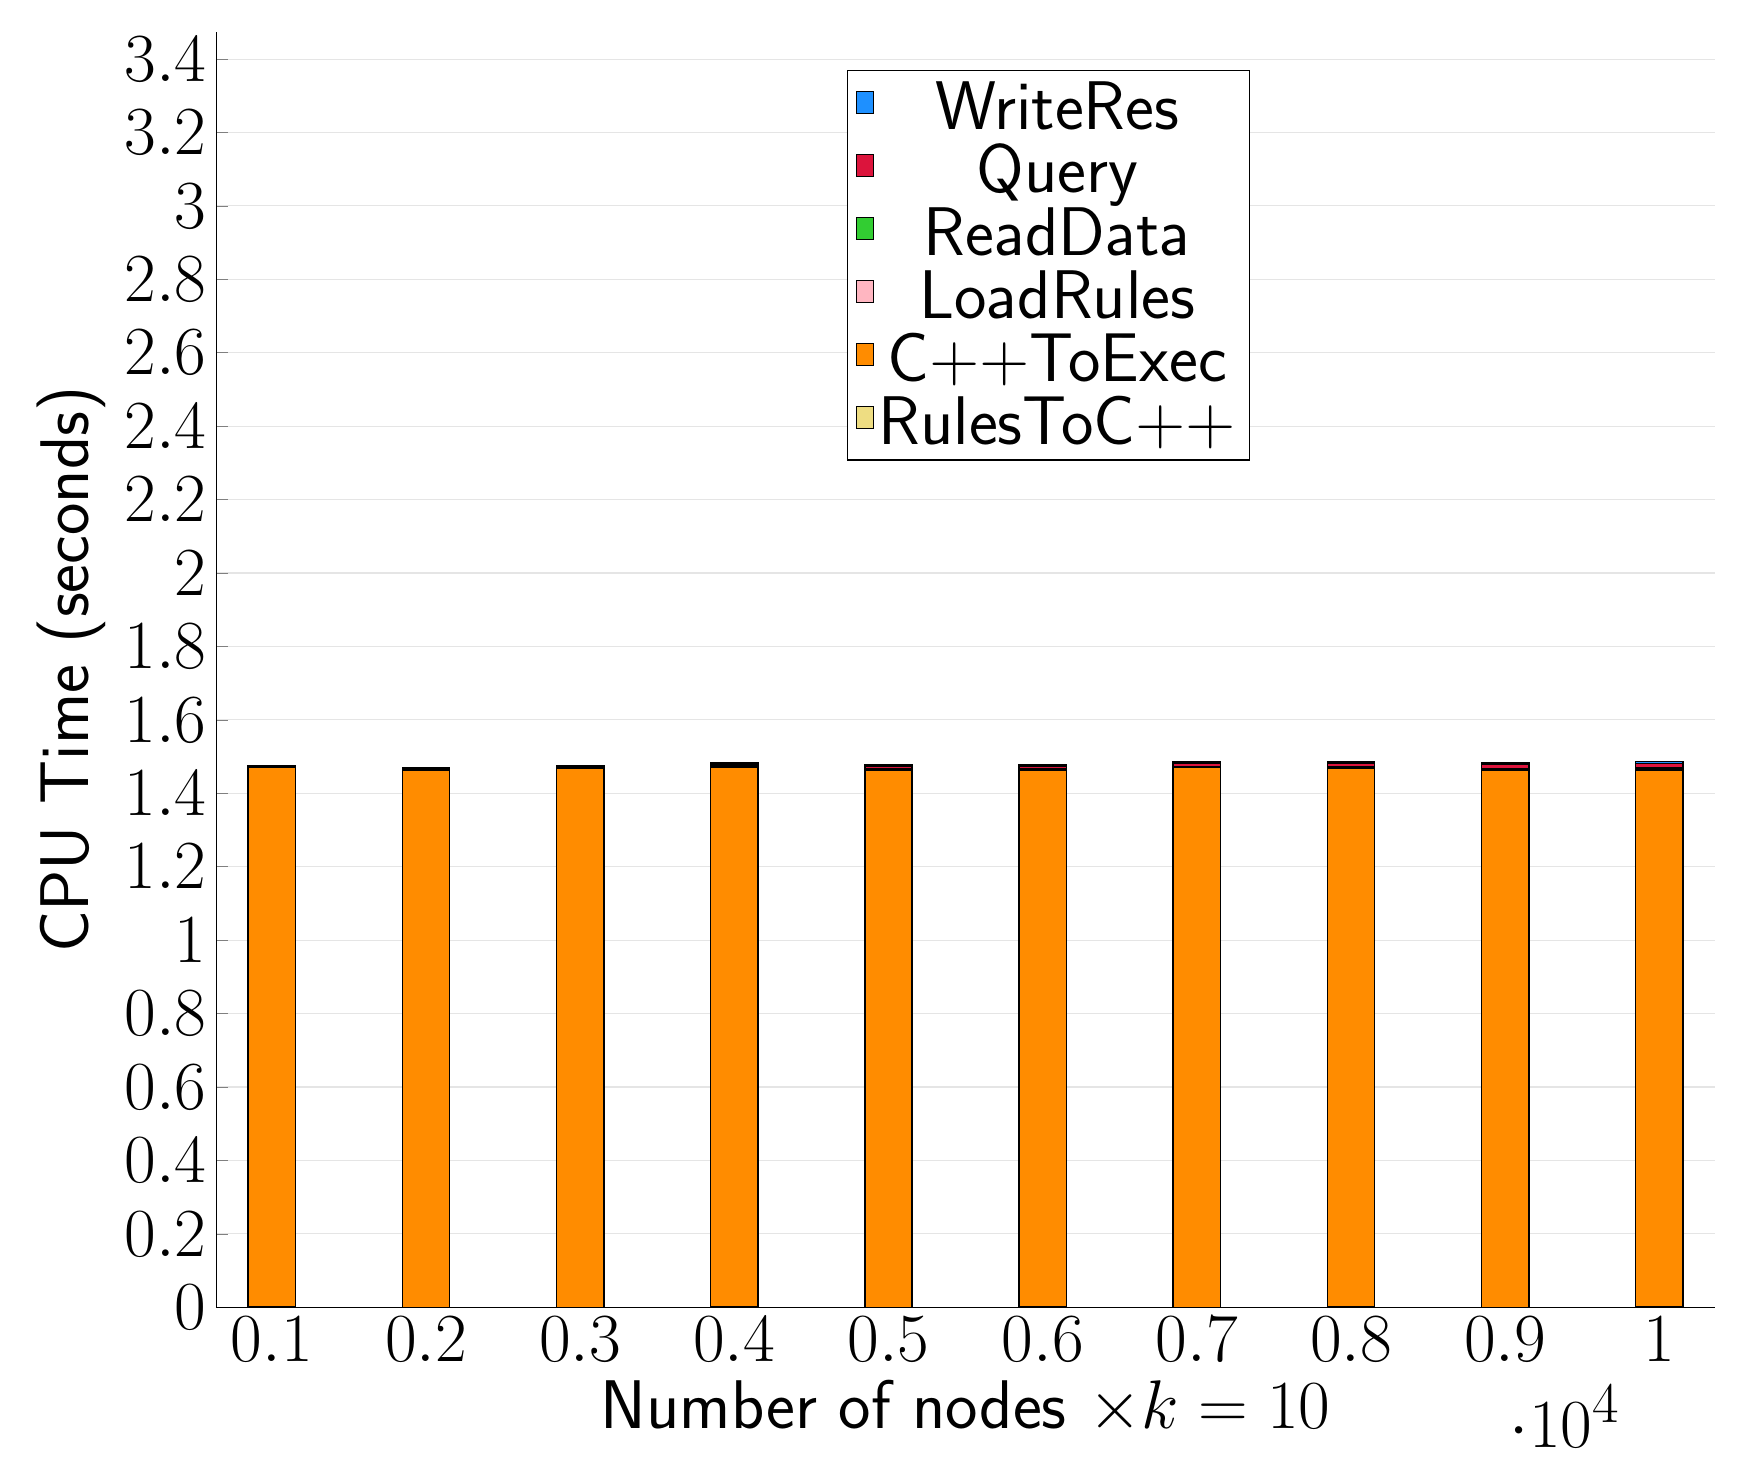
\begin{tikzpicture}
\begin{axis}[
   ybar stacked,
   width=1.7\textwidth,
   bar width=0.6cm,
   ymajorgrids, tick align=inside,
   major grid style={draw=gray!20},
   xtick=data,
   ymin=0, ymax=3.474,
   axis x line*=bottom,
   axis y line*=left,
   enlarge x limits=0.04,
   legend style={
       at={(0.69, 0.97)},
       anchor=north east,
       legend columns=1,
       font=\Huge,
   },
   ylabel={CPU Time (seconds)},
   xlabel={Number of nodes $\times k=10$},
   label style={font=\Huge},
   tick label style={font=\Huge},
]
\addlegendimage{fill=DodgerBlue, draw=black, line width=0.2pt}
\addlegendentry{WriteRes}
\addlegendimage{fill=Crimson, draw=black, line width=0.2pt}
\addlegendentry{Query}
\addlegendimage{fill=LimeGreen, draw=black, line width=0.2pt}
\addlegendentry{ReadData}
\addlegendimage{fill=LightPink, draw=black, line width=0.2pt}
\addlegendentry{LoadRules}
\addlegendimage{fill=DarkOrange, draw=black, line width=0.2pt}
\addlegendentry{C++ToExec}
\addlegendimage{fill=LightGoldenrod, draw=black, line width=0.2pt}
\addlegendentry{RulesToC++}
\addplot +[fill=LightGoldenrod, draw=black, line width=0.55pt] coordinates {
(1000, 0.0020000000000000005)
(2000, 0.0)
(3000, 0.0)
(4000, 0.0020000000000000005)
(5000, 0.0)
(6000, 0.0020000000000000005)
(7000, 0.0)
(8000, 0.0020000000000000005)
(9000, 0.0)
(10000, 0.0020000000000000005)
};
\addplot +[fill=DarkOrange, draw=black, line width=0.55pt] coordinates {
(1000, 1.468)
(2000, 1.462)
(3000, 1.468)
(4000, 1.47)
(5000, 1.464)
(6000, 1.462)
(7000, 1.47)
(8000, 1.4659999999999997)
(9000, 1.464)
(10000, 1.462)
};
\addplot +[fill=LightPink, draw=black, line width=0.55pt] coordinates {
(1000, 0.000149)
(2000, 0.0001604)
(3000, 0.0001636)
(4000, 0.000155)
(5000, 0.00016000000000000004)
(6000, 0.00014759999999999998)
(7000, 0.00015900000000000002)
(8000, 0.0001524)
(9000, 0.0001628)
(10000, 0.0001524)
};
\addplot +[fill=LimeGreen, draw=black, line width=0.55pt] coordinates {
(1000, 0.0008867999999999999)
(2000, 0.0012736)
(3000, 0.00162)
(4000, 0.0020811999999999996)
(5000, 0.0023436)
(6000, 0.0025222)
(7000, 0.0029387999999999997)
(8000, 0.0033607999999999997)
(9000, 0.0038582)
(10000, 0.0043684)
};
\addplot +[fill=Crimson, draw=black, line width=0.55pt] coordinates {
(1000, 0.0016308000000000004)
(2000, 0.0031287999999999997)
(3000, 0.0044632)
(4000, 0.0057698)
(5000, 0.0071826)
(6000, 0.0077234)
(7000, 0.009251)
(8000, 0.010501400000000001)
(9000, 0.011587)
(10000, 0.012884399999999999)
};
\addplot +[fill=DodgerBlue, draw=black, line width=0.55pt] coordinates {
(1000, 0.0012553999999999998)
(2000, 0.0018254)
(3000, 0.0021016)
(4000, 0.0025834000000000005)
(5000, 0.0031742)
(6000, 0.0030274)
(7000, 0.0038598)
(8000, 0.0041329999999999995)
(9000, 0.0046658)
(10000, 0.0050278)
};
\end{axis}
\end{tikzpicture}

\end{document}
